% Source: Analysis_CODES/fitER/results/comparisons/punzi_count_slides; accepted numerical intake 20260920.
\begin{frame}[label=p23_20260920]{Punzi optimization: resolve the relevant efficiency range}
\textbf{Henrique's suggestion:} scan score cuts from 0.05 to 0.95 in steps of 0.05.
\[
 \mathrm{FOM}(t)=\frac{\epsilon_{\mathrm{MC}}(t)}{a/2+\sqrt{B(t)}},
 \qquad a=5,\qquad B(t)=\frac{N_{\mathrm{left}}(t)+N_{\mathrm{right}}(t)}{3}.
\]
\begin{itemize}\small
\item $\epsilon_{\mathrm{MC}}$: fraction of weighted MC passing score $>t$, within $3.62<m<4.00$ GeV; weight = \var{pThatreweight}.
\item Signal window: $[3.84,3.90]$ GeV; sidebands: $(3.75,3.84)$ and $(3.90,3.99)$ GeV. Window acceptance factor = 1.
\item $B$: unit-weight DATA sideband counts, scaled by the window-width ratio; linear-background approximation.
\item \textbf{xeff}: weighted reference-MC passing fraction without the mass cut; used to set the scan thresholds.
\end{itemize}
\takeaway{Fine scan: target xeff 15\%--60\% in 1\% steps (46 points).\newline Coarse score scan: only 4 points in this efficiency range.}
\caution{Shown errors include sideband counting statistics only. The 260916 $S/\sqrt{S+B}$ scan used a different definition.}
\end{frame}

\begin{frame}[label=p24_20260920]{9v9: coarse and fine Punzi scans versus score}
\begin{columns}[T]
\column{0.49\textwidth}\centering\textbf{Coarse score scan}\par
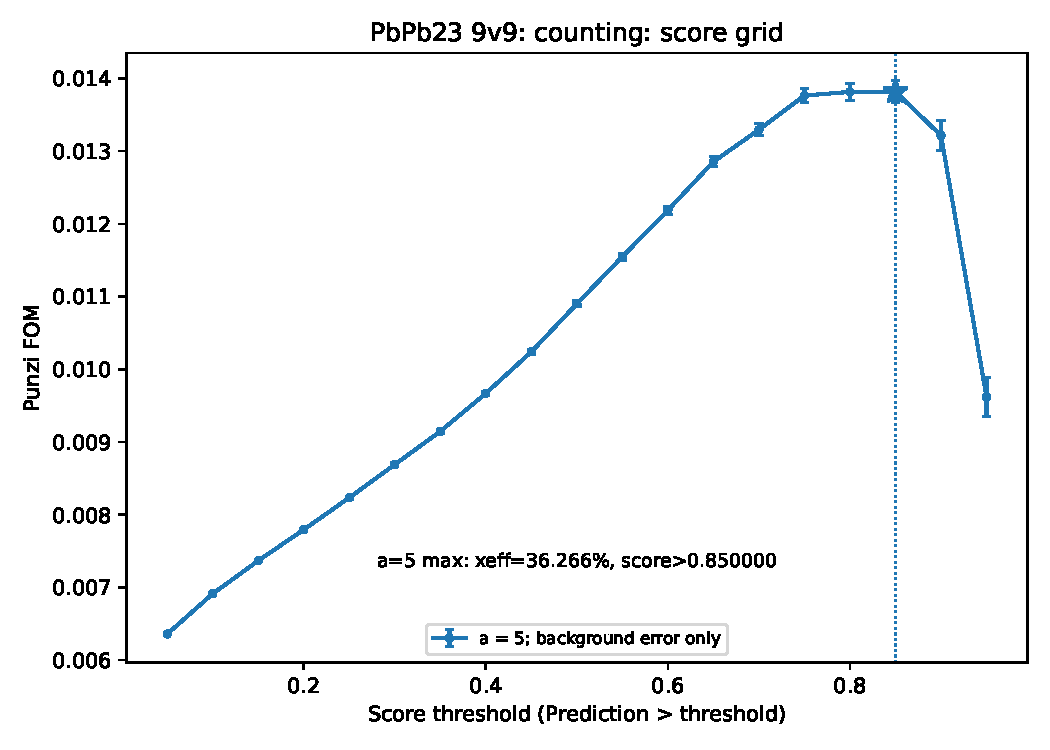
\includegraphics[width=\linewidth,height=0.56\textheight,keepaspectratio]{figures/20260920/punzi/9v9_score_scan_vs_score.pdf}
\column{0.49\textwidth}\centering\textbf{Fine xeff scan}\par
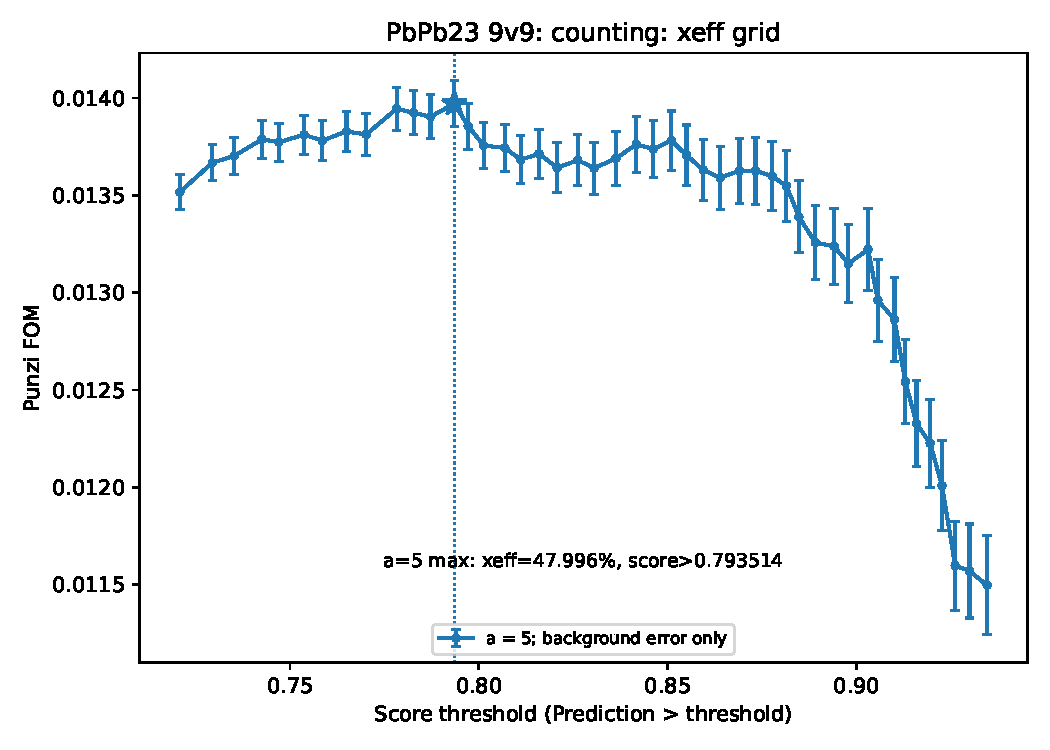
\includegraphics[width=\linewidth,height=0.56\textheight,keepaspectratio]{figures/20260920/punzi/9v9_xeff_scan_vs_score.pdf}
\end{columns}
\begin{itemize}\small
\item Coarse-grid maximum: score $0.85$, xeff $36.27\%$; agrees with Henrique's reported cut.
\item Fine-grid maximum: score $0.793514$, target xeff $48\%$; missed by the coarse grid.
\end{itemize}
\caution{Agreement concerns the coarse-grid maximum; Henrique's full original settings are unavailable.}
\end{frame}

\begin{frame}[label=p25_20260920]{9v9: efficiency spacing explains the coarse-scan limitation}
\begin{columns}[T]
\column{0.49\textwidth}\centering\textbf{Coarse score scan}\par
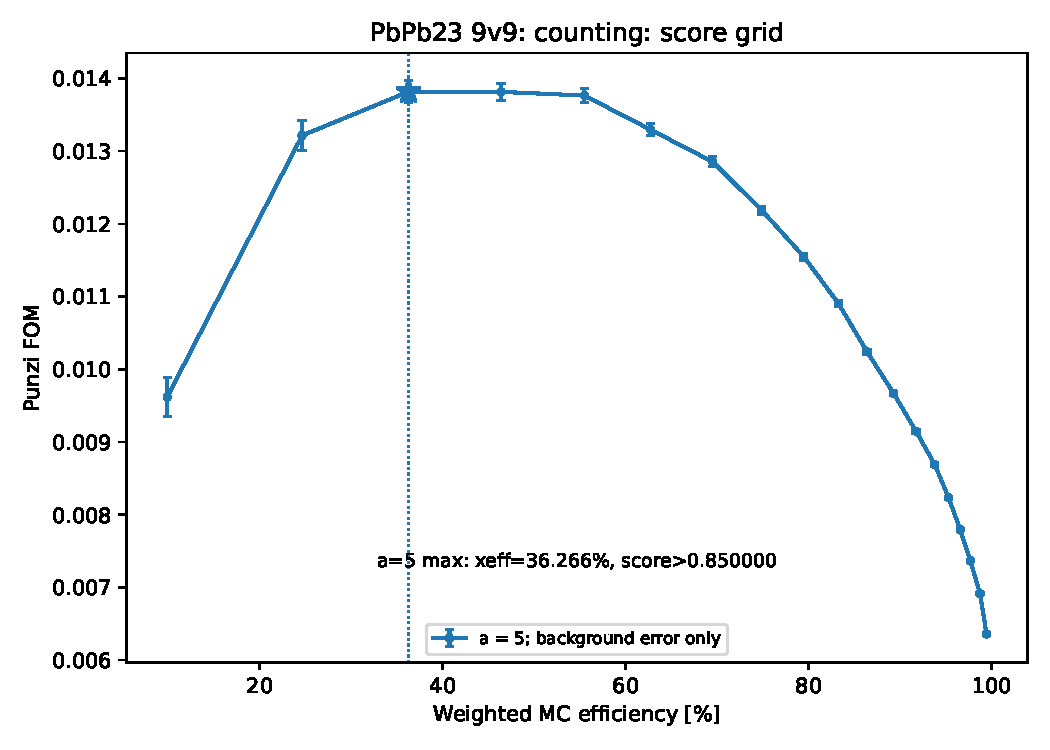
\includegraphics[width=\linewidth,height=0.56\textheight,keepaspectratio]{figures/20260920/punzi/9v9_score_scan_vs_xeff.pdf}
\column{0.49\textwidth}\centering\textbf{Fine xeff scan}\par
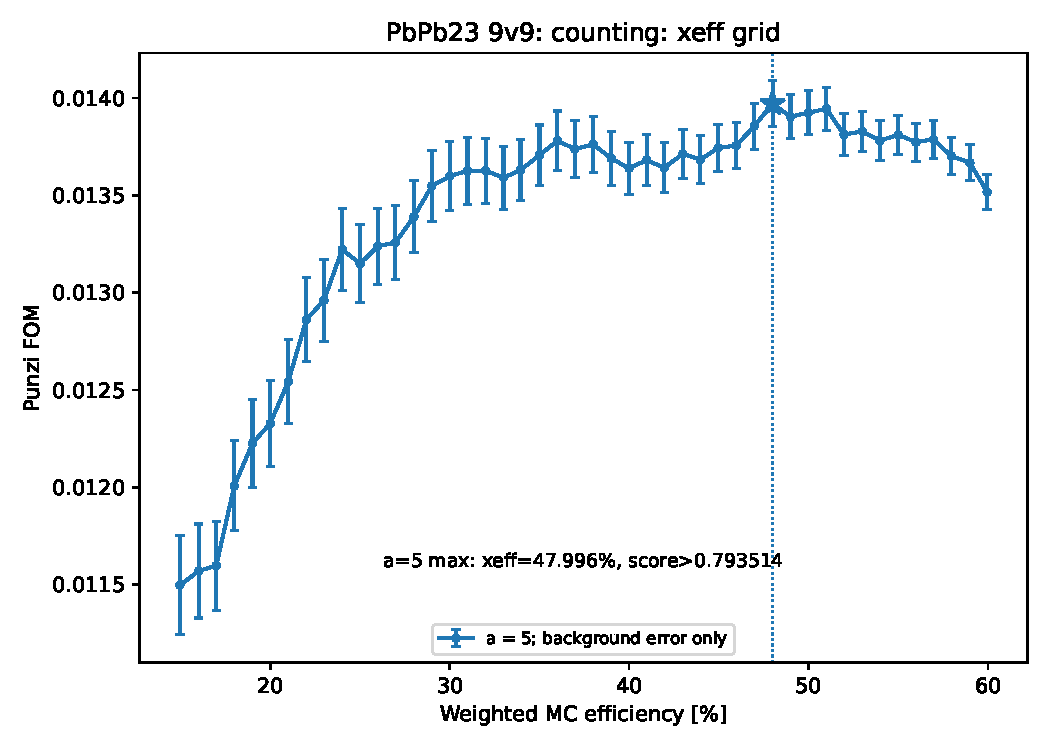
\includegraphics[width=\linewidth,height=0.56\textheight,keepaspectratio]{figures/20260920/punzi/9v9_xeff_scan_vs_xeff.pdf}
\end{columns}
{\small Coarse points in the chosen range: xeff $24.64,\ 36.27,\ 46.39,\ 55.49\%$.\par
Fine-scan maximum: $48\%$; points above 99\% of peak FOM: $47$--$51\%$.}
\takeaway{Interim conclusion: scan in xeff to resolve the relevant efficiency range and the Punzi plateau.}
\end{frame}
